\chapter{Architecture}
\label{cha:architecture}

This chapter is dedicated to displaying and describing the numerous components,
their relationships, and the general needs for the cluster architecture's composition.
\\ %
Understanding how the cluster works lays a good foundation for the following chapters,
in which almost everything seen here is extensively explained in terms of how it
was developed and why certain decisions were taken. Furthermore, the design is
dynamic and may be modified to include more or fewer components and/or
requirements to better meet the requirements of the end user. \\ %
Section \ref{subsec:architecture_cluster_example} depicts a real-world
functioning example of the cluster design given. \\ %
It has been extensively tested and is continuously operational 24 hours a day, hosting
a variety of services. Furthermore, it upscales or downscales automatically dependent
on demand or requirements. \\ %
The diagram below illustrates the architecture, encompassing its components and
how they are interconnected, as well as a potential connection to an external network.

\begin{figure}[htbp]
  \centering
  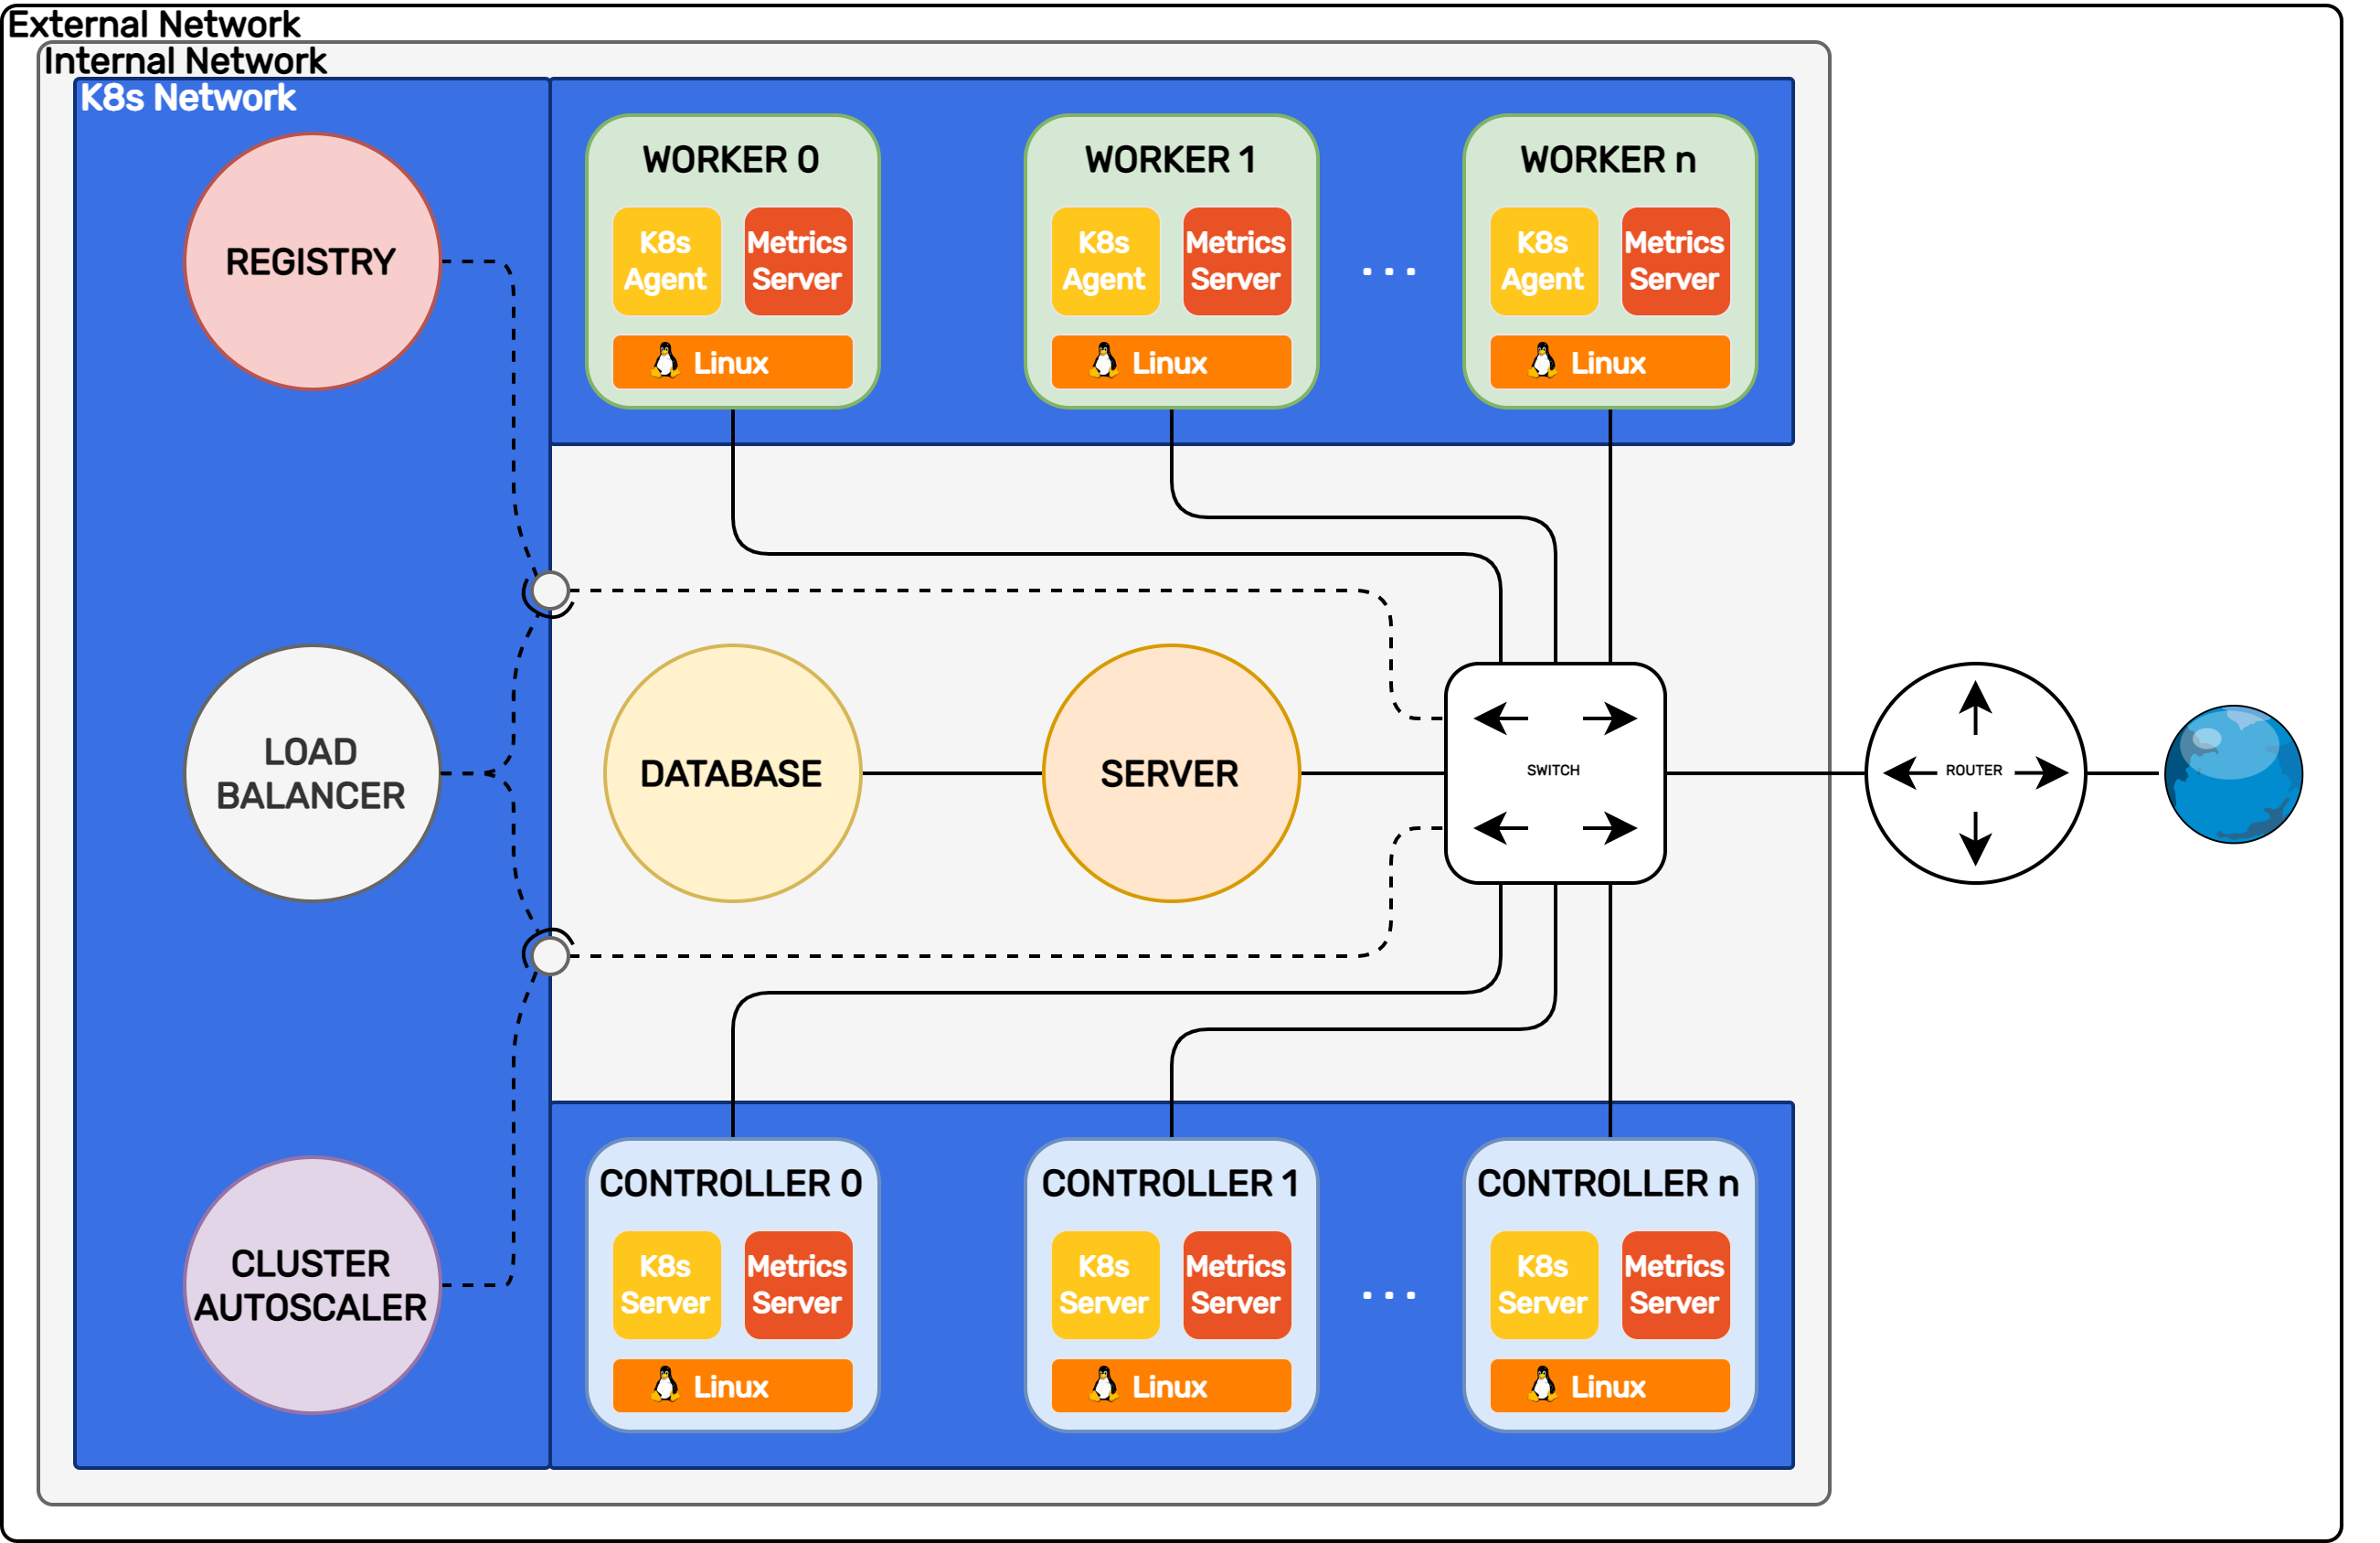
\includegraphics[width=\textwidth]{images/recluster/architecture.png}
  \caption{Architecture overview}
\end{figure}

\section{Components}
\label{sec:architecture_components}

\subsection{Node}
\label{subsec:architecture_components_node}

A node is a physical computer that runs the \texttt{Linux Kernel} and constantly
executes software that is specific to the cluster's composition. Linux is a
clone of the operating system Unix\footnote{\url{https://unix.org}}, written from
scratch by Linus Torvalds\footnote{\url{https://wikipedia.org/wiki/Linus_Torvalds}}
with help from a loosely-knit team of hackers across the world. It aims towards
POSIX and Single UNIX Specification compliance\cite{linux}.\\ %
Each node is physically connected to the other nodes via Ethernet and to the
many operating services/components through a virtual network. Section \ref{sec:architecture_network}
goes into further detail about cluster networking. \\ %
A node can be in one of two states. The \texttt{active} state indicates that a node
is turned on and is actively contributing to the cluster. The \texttt{inactive} state,
on the other hand, shows that a node has been turned off and is no longer actively
contributing to the cluster. This does not imply that the node is worthless and
will never be utilized again, but simply that it is no longer required for the current
cluster demand. A node state can be changed manually by switching the power
button on or off, or automatically through the Cluster Autoscaler component,
which monitors the current cluster state. More details about Cluster Autoscaler may
be found in section \ref{subsec:architecture_components_cluster_autoscaler}. \\ %
% TODO Maybe K8s reference section ?
Two core services are continuously operating on each node. The first service is
a Kubernetes-compliant distribution. Kubernetes, also known as K8s, is an open-source
solution for automating containerized application deployment, scaling, and administration\cite{k8s}.
The second service, Metrics Server, is a server that constantly monitors the node,
exposing hardware and operating system metrics. \\ %
Finally, each node is conceptually divided into two types depending on its role in
the cluster: Worker nodes and Controller nodes. These are discussed in the sections
that follow.

\subsubsection{Worker}
\label{subsubsec:architecture_components_node_worker}

\begin{wrapfigure}
  {l}{0pt} %
  \raisebox{0pt}[\dimexpr\height-\baselineskip\relax]{\centering
  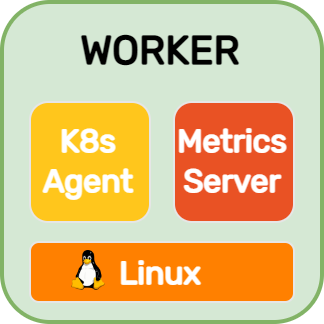
\includegraphics[width=.2\textwidth]{images/recluster/worker.png}}%
\end{wrapfigure}

A worker node is designed to handle only deployable units of computation and services
that are not critical components of the cluster. It is not in charge of
scheduling the work over several nodes; rather, it only accepts it from a
cluster-available authenticated and authorized controller node. \\ %
Even though a worker node executes the effectively scheduled workload in the
cluster, it is not considered a critical component of it. At any given time, the
total number of active workers might be zero. That is, there is no scheduled workload,
and previously worker nodes have been shut down automatically to prevent
precious resource waste that is no longer required. \\ %
The majority of the cluster's accessible machines are worker nodes. This raises the
overall amount of schedulable workload as well as heterogeneity. Heterogeneity
is helpful because it may help schedule workloads to nodes with the bare minimum
of requested resources, preventing waste. Assume that the total number of
\texttt{active} nodes in the cluster is zero and that there are two \texttt{inactive}
worker nodes. The first node has 4 GiB of memory and consumes 100W of power,
whereas the second node has 8 GiB of memory and consumes 150W of power. A workload
using around 3GiB of memory is then planned for the cluster. Because it
decreases resource waste, notably memory waste, the first worker node will be
chosen. It is important to note that if both nodes have an equal amount of memory,
the conclusion remains the same since it has the lowest power consumption.

\subsubsection{Controller}
\label{subsubsec:architecture_components_node_controller}

\begin{wrapfigure}
  {l}{0pt} %
  \raisebox{0pt}[\dimexpr\height-\baselineskip\relax]{\centering
  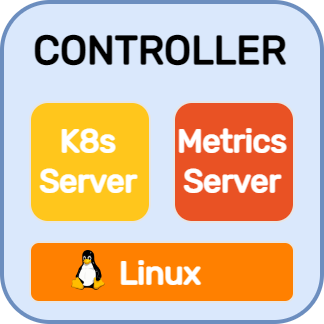
\includegraphics[width=.2\textwidth]{images/recluster/controller.png}}%
\end{wrapfigure}

The total number of \texttt{active} or \texttt{inactive} nodes in the cluster is
not limited. However, a large number of nodes increases the workload on
controller nodes, which must maintain the cluster state updated and synchronized.
As a result, as shown in table \ref{tbl:controller_node_requirements}\cite{k3s_requirements},
their quantity and hardware requirements must be carefully balanced.

\begin{xltabular}
  {\textwidth} { c | >{\ttfamily}c | >{\ttfamily}c | >{\ttfamily}c }

  \multicolumn{1}{ c |}{\large{\textbf{Deployment Size}}} &
  \multicolumn{1}{ c |}{\large{\textbf{Nodes}}} &
  \multicolumn{1}{ c |}{\large{\textbf{Cores}}} &
  \multicolumn{1}{ c}{\large{\textbf{Memory}}} \\ \hline \hline

  Small & \char`~ 10 & 2 & 4 GiB \\ \hline

  Medium & \char`~ 100 & 4 & 8 GiB \\ \hline

  Large & \char`~ 250 & 8 & 16 GiB \\ \hline

  X-Large & \char`~ 500 & 16 & 32 GiB \\ \hline

  XX-Large & 500+ & 32 & 64 GiB \\

  \caption{Controller node requirements based on cluster size}
  \label{tbl:controller_node_requirements}
\end{xltabular}

\subsection{Server}
\label{subsec:architecture_components_server}

\subsection{Database}
\label{subsec:architecture_components_database}

\subsection{Registry}
\label{subsec:architecture_components_registry}

\subsection{Cluster Autoscaler}
\label{subsec:architecture_components_cluster_autoscaler}

\subsection{Load Balancer}
\label{subsec:architecture_components_load_balancer}

\section{Network}
\label{sec:architecture_network}

\subsection{Overlay Network}
\label{subsec:architecture_network_overlay_network}

\subsection{Domain}
\label{subsec:architecture_network_domain}

\section{Cluster}
\label{sec:architecture_cluster}

\begin{wrapfigure}
  {r}{.5\textwidth}
  \centering
  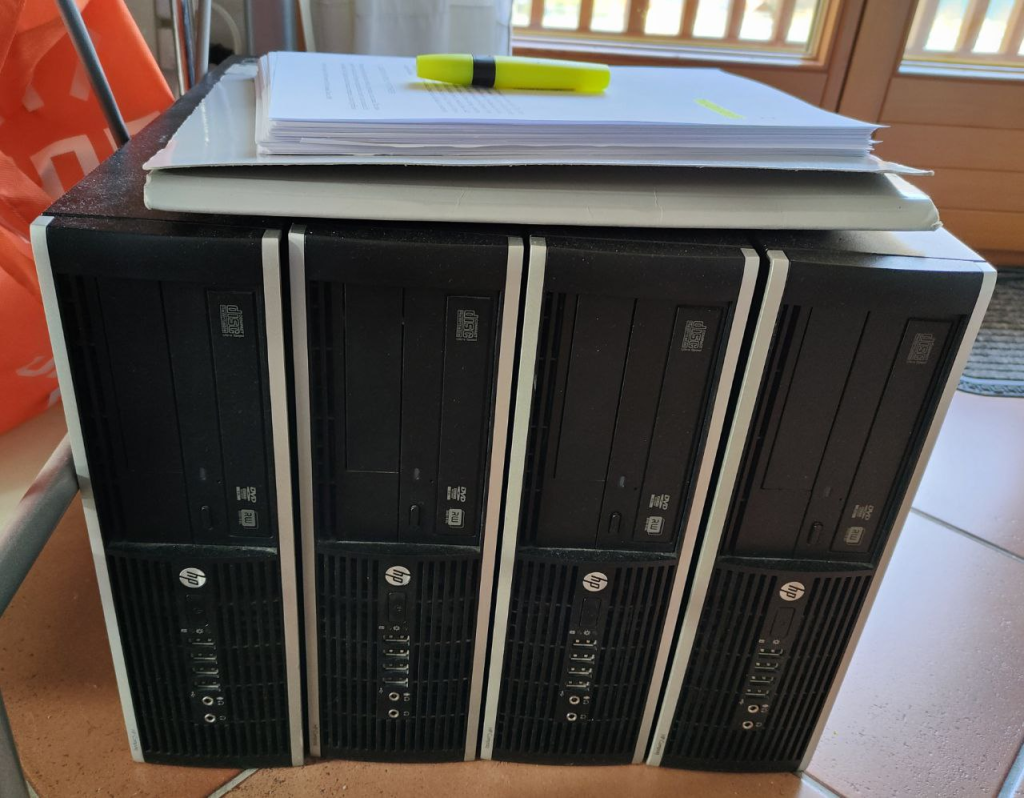
\includegraphics[width=.5\textwidth]{images/recluster/cluster.png}
  \caption{reCluster cluster}
\end{wrapfigure}

\subsection{Hardware}
\label{subsec:architecture_cluster_hardware}

% TODO WoL features, how to turn on nodes
% TODO Prefer nodes with WoL upscaling

\subsection{Example}
\label{subsec:architecture_cluster_example}

% TODO Move